%theoretical.tex
% Theoretical Background %

\section{Ab Initio Many Body Quantum Mechanics}
 The first task of quantum chemistry is to formulate mathematics that can describe molecular systems through the physics of non-relativistic electrons and nuclei. This is accomplished through Hamiltonian mechanics acting on a set of functions, a basis, dubbed the Schr{\"o}dinger equation.
   \begin{equation}
    \hat{H}\ket{\Psi} = E\ket{\Psi}
   \end{equation}
 This equation represents a multi variable partial differential equation where the Hamiltonian represents the kinetic plus the potential energy operator of a system.  For the time-independent Schr{\"o}dinger equation the full Hamiltonian is formed in the lens of electrostatic interactions of electrons and nuclei.  This formulation brings about the first approximation in quantum mechanics, the Born-Oppenheimer approximation.\cite{Szabo 1996}  Because of the difference in mass between nuclei and electrons, there is a disparity in their relative motion.  Thus one can decide to gauge the full problem in the realm of either a fixed nuclear field with point charge electron coordinates or an average field of electronic charge with nuclei embedded within. To be consistent with the mathematic formulation of electronic structure theory this paper will only consider the problem of explicit electrons coordinate systems with fixed nuclear position.  The approximation allows one to reduce the terms in the full Hamiltonian, allowing one to neglect the kinetic energy of nuclei and consider nuclear-nuclear repulsion as a constant.  What is left is the N-body electronic Hamiltonian
   \begin{equation}
    \hat{H}_{elec} = -\sum_{i=1}^{N} \frac{1}{2} \nabla_{i}^{2} - \sum_{i=1}^{N}\sum_{A=1}^{M} \frac{Z_A}{r_{iA}} + \sum_{i=1}^{N}\sum_{j>i}^{N} \frac{1}{r_{ij}}
   \end{equation}
  The first term in this expression is the kinetic energy operator applied to N electrons, the second is the potential energy operator between electron-nuclei pairs and the final term is the potential energy operator of electron-electron pairs.  This Hamiltonian can be used to solve the electronic Scr{\"o}dinger equation
    \begin{equation}
     \hat{H}_{elec} \ket{\Psi_{elec}} = E_{elec}\ket{\Psi_{elec}}
    \end{equation}
  With the electronic wave function, $\Psi_{elec}$, dependent explicitly on the position of electrons and implicitly on the position of the nuclei.  Because $E_{elec}$ depends parametrically on the position of the nuclei, the total energy of the system can be calculated as 
    \begin{equation}
      E_{tot} = E_{elec} + \sum_{A=1}^{M} \sum_{B>A}^{M} \frac{Z_A Z_B}{R_{AB}}
    \end{equation}
  The nuclear repulsion term can be considered after the differential equation because it will only scale the eigenvalues of the expression.  Though the full multi variable partial differential Schr{\"o}dinger equation defined above is simplified with the Born-Oppenheimer approximation, it is still too complicated to solve for systems with more than one electron.\cite{Szabo 1970}

  %%%%%%%%%%%%%%%%%%%%%%%%%%%%%%%%

  \subsection{Hartree-Fock}
    Though it may not be possible to analytically solve the Schr{\"o}dinger equation for an arbitrary number of electrons, it is able to exactly solve the differential for one electron.  Since the Hamiltonian operator is a linear operator, the concept of solving the Schr{\"o}dinger equation in a basis of N-tuple single electron functions is the fundamental basis for approximate numerical solutions, known as Hartree-Fock theory. \cite{Hartree 1928, Fock 1930, Szabo 1996, Sherril 2000} This approximation implies that one can express the electronic wave function, $\Psi_{elec}$, as a product of one electron functions that depend on the coordinate, $x = \{r, \omega\}$, which contains spacial, r, and spin, $\omega$, coordinates. In order to provide a physically accurate description of electrons, the product solution to the electronic wavefunction must be antisymmetric with respect to the interchange of coordinates, x, of any two electrons.  Formally the antisymmetric principle can be enforced with the introduction of Slater determinants\cite{Slater 1929, Slater 1930} 

    \begin{equation}
    \Psi_{0}(x_1, x_2, ..., x_N) = \frac{1}{\sqrt{N!}}
    \begin{vmatrix}
     \chi_i(x_1) &\chi_j(x_1) &\ldots   &\chi_k(x_1)   \\
     \chi_i(x_2) &\chi_j(x_2)  &\ldots & \chi_k(x_2)   \\
     \vdots&\vdots   &\vdots &\vdots   \\
     \chi_i(x_N) &\chi_j(x_N) & \ldots & \chi_k(x_N)
    \end{vmatrix}
    \end{equation}

    Through the act of creating a wavefunction via a Slater determinant one introduces exchange correlation to electrons characterized by the same spin variable.  Though electrons of opposite spin are a simple uncorrelated product of one another.\\
    The best, lowest energy approximation to the Schr{\"o}dinger solution is found variationally, by minimizing the one electron spin orbitals via the Rayleigh quotient
      \begin{equation}
      E_{0} = \frac{\bra{\Psi_{0}} \hat{H}_{elec} \ket{\Psi_{0}}}{\selfolap{\Psi_{0}}}
      \end{equation}
    held to the constraint that $\olap{ \chi_i}{\chi_j} = \delta_{ij}$ where $\delta_{ij}$ is the kronecker delta such that $\delta_{ij}=1\iff i=j$ else $\delta_{ij} = 0$ and where the bracket notation implies the Hilbert space inner product.  The inner product $\bra{\Psi_{o}} \hat{H}_{elec} \ket{\Psi_{0}}$ is a set of eigenvalue integro-differential equation over all space, the Hartree-Fock equations, with each element defined as 
      \begin{equation}
      \hat{f}\chi_i = \epsilon_i \chi_i
      \end{equation}
    $\hat{f}$ the Fock operator is an effective one-electron operator of the form 
      \begin{equation}
      \hat{f}(x_1) = \hat{h}_i(x_1)  + \sum_{j\neq i}^N \hat{J}_j(x_1) - \hat{K}_j(x_1)
      \end{equation}
    where $\hat{h}(x_1)$ is the average kinetic and nuclear attraction energy of a single electron and is expressed as 
      \begin{equation}
      \hat{h}(x_1) = -\frac{1}{2} \nabla_1^2 - \sum_{A=1}^M \frac{Z_A}{r_{1A}}
      \end{equation}
    The last two terms in equation (8) represent the potential energy of the electron-electrons interaction.  The first term $\hat{J}_j$ is the classical coulombic repulsion between two electrons or equivalently the average local potential at $x_1$ arising from an electron in $\chi_j$
      \begin{equation}
      \hat{J}_j(x_1) = \int \chi_j^*(x_2) \frac{1}{r_{ij}} \chi_j(x_2) dx_2
      \end{equation}
    The second term $\hat{K}_j$ is referred to as the exchange term does not have a classical representation as the previous terms do, it is a direct product of the antisymmetric nature of the single determinant wave function and is defined as 
      \begin{equation}
      \hat{K}_j(x_1) = \int \chi_j^*(x_2) \frac{1}{r_{ij}} \chi_i(x_2) dx_2
      \end{equation}
    As mentioned previously the exchange term allows Hartree-Fock methods to recover correlation energy from electrons with opposite spins, though same spin electrons are still uncorrelated.  \\
    The solution of this Hartree-Fock eigenvalue equation provides a set of $\{ \chi_k \}$ orthonormal spin orbitals each with orbital energy $\{\epsilon_k\}$.  In principle there are infinitely many solutions to the Hartree-Fock equation.  Though in a finite basis of spin orbitals there exists K spatial orbitals giving rise to 2K spin orbitals.  The solution of the Hartree-Fock eigenvalue problem consist of N occupied and 2K-N unoccupied orbitals.  Larger basis sets variationally reduce the Hartree-Fock Energy, $E_0$, to the Hartree-Fock limit and will be useful in methods such as configuration interaction and coupled cluster.\cite{Szabo 1996}  \\
    Finally in order to numerically solve the Hartree-Fock eigenvalue equation one must provide a solution for the one electron orbital functions $\{\chi_k\}$.  From solutions of the Schr{\"o}diger's equation applied to the Hydrogen atom, it is well understood that Slater type orbitals can describe one electron orbitals exactly.  Both the numerical differentiation and integration of Slater type orbitals as well as finding a different distinct functional solution to the Hartree-Fock equations provide a formidable challenge. In order to produce a simplified solution one expands the one electron basis function into an M function atomic orbital basis
      \begin{equation}
      \chi_i = \sum_\mu^M C_{i\mu} \phi_\mu(x)
      \end{equation}
    where $\phi_\mu$ are typically atom centered functions.  Applying the transformation into equation (7) produces what is known as the Hartree-Fock-Roothaan equation\cite{Roothaan 1960, Roothaan 1951}, the matrix equation being 
      \begin{equation}
      \textbf{FC} = \textbf{SC}\epsilon
      \end{equation}
    \textbf{C} is an M x N matrix of coefficients which describe the transformation in equation (12).  In equation (11), \textbf{S} is the overlap of two atomic orbitals
      \begin{equation}
      S_{\mu\nu} = \int \phi^*_\mu(x_1) \phi_\nu(x_1) dx_1
      \end{equation}
    The elements of the Fock matrix, \textbf{F}, are
      \begin{equation}
      F_{\mu\nu} = \int \phi_\mu(x_1) \hat{f}(x_1) \phi_\nu(x_1) 
      \end{equation}
    The Fock matrix terms can also be expanded with respect to the operators defined in equations (9-11):
      \begin{equation}
      F_{\mu\nu} = h_{\mu\nu} + \sum_{occ}\sum_{\rho \sigma} C_{\rho i} C_{\sigma i} \bra{\mu \rho}\ket{\nu \sigma}
      \end{equation}
    where 
      \begin{equation}
      \bra{\mu \rho}\ket{\nu \sigma} = \olap{\mu \rho}{\nu \sigma} - \olap{\mu \rho}{\sigma \nu}
      \end{equation}
    is the antisymmetrized difference of the coulomb and exchange terms with 
      \begin{equation}
      \olap{\mu \rho}{\nu \sigma} = (\mu \nu | \rho \sigma) = \int \int \phi^*_\mu(x_1) \phi^*_\rho(x_2) \frac{1}{r_{12}} \phi_\nu (x_1) \phi_\sigma(x_2) dx_1 dx_2
      \end{equation}
    being the two-electron integrals in physicist and chemist notation, respectively. In the computational procedure of Hartree-Fock, evaluation of the Fock matrix is the most expensive step with asymptotic scaling of $\mathcal{O}(N^4)$ where N is the number of electrons. Because of the basis expansion in the development of Roothaan's equation, the system of equations is non-linear and must be solved iteratively to calculate the optimal expansion coefficients, this is achieved via the self-consistent-field (SCF) procedure.

  %%%%%%%%%%%%%%%%%%%%%%%%%%%%%%%%

  \subsection{Electronic Correlation Methods}
    Correlation is a concept of probability in that two variables are considered independent if the joint probability of the variables is a product of each variables probability; $p(x,y) = p(x) \times p(y)$ where $p(\cdot)$ is a probability function.  Else, the two variables are said to be correlated.\cite{Kutzelnigg 2003}  Electron correlation is mainly established because from antisymmetric and indistinguishable properties of fermion electrons and Coulombic repulsion between electronic charges. Hartree-Fock does cannot recover electron correlation beyond the fermionic portion discussed previously.  The wave function in Hartree-Fock theory relies on the independent particle model, by definition this is an uncorrelated description,  and it does not consider electron-electron repulsion explicitly but as electron repulsion with an average electron cloud charge.  Correlation energy, as defined by L{\"o}wdin \cite{Lowdin 1959}, is 
      \begin{equation}
      E_{corr} = \mathcal{E}_{0} - E_{HF}
      \end{equation}
    Where $\mathcal{E}_0$ is the exact non-relativistic energy and $E_{HF}$ energy recovered at the Hartree-Fock limit.  This definition is imprecise, so it may be more useful to think of $E_{corr}$ as an observable of some quantum mechanical operator acting on wave function with the form:
      \begin{equation}
      \Psi_{exact} = \Psi_{HF} + \Psi_{corr}
      \end{equation}
    where $\Psi_{corr}$ is orthogonal to $\Psi_{HF}$ and encapsulates all correlation not captured by Hartree-Fock.\cite{Kong 2012}  Though correlation only contributes a very small portion to the total energy of a molecule, these corrections are extremely necessary in the accurate calculation of molecular properties and prediction of reactions.  Outlined to follow are a few methods that allow theoretical chemistry to systematically calculate correlation energy.

    %Find that electron repulsion picture that fabijan used.

    %%%%%%%%%%%%%%%%%%%%%%%%%%%%%%%%

    \subsubsection{Many Body Perturbation Theory}
      Many Body Perturbation Theory (MBPT) was first developed in 1957\cite{Brueckner, 1955} to study the energy of nuclear matter.  Not until 1968 was the it applied to ab initio quantum chemistry.\cite{Freed 1968, Freed 1971}.  Though there are many formulations of MBPT, two of the most well known being Rayleigh-Schr{\"o}dinger\cite{Lindgren 1974} and M{\/o}ller-Plesset\cite{Moller 1934, Raghavachari 1989}, all methods are developed from the same principles.  The distinction comes from the use of diagrams and the definition of the zeroth order hamiltonian and perturbative potential.  The formulation presented will follow the M{\/o}ller-Plesset (MPn) definition of MBPT, where n is the perturbative order correction. MBPT is not variational, the solution recovered from an approximation is lower bounded by the exact energy, but is size consistent. For a method to be size consistent it must be able to calculate the energy of two elements, separated by infinite distant to be the sum of its individual parts.  
        \begin{equation}
        	E_{r=\infty}(AB) = E(A) + E(B)
        \end{equation}
      The full wavefunction and energy term of the eigenvalue problem 
        \begin{equation}
        	\hat{H}_{elec}\ket{\Phi} =  E\ket{\Phi}
        \end{equation}
      can be expanded with the MBPT hamiltonian
      \begin{equation}
      	\hat{H}_{elec} = \hat{H}^{(0)} - \lambda \hat{H}^{(1)}
      \end{equation}
      Where $\hat{H}^{(0)}$, the zeroth order hamiltonian, is assumed to very closely approximates the exact hamiltonial; $\hat{H}^{(1)}$ is the perturbative, first order correction to the zeroth order problem and the perturbative wave function and energy expansions
        \begin{equation}
        	\ket{\Phi} = \ket{\Phi^{(0)}} + \lambda \ket{\Phi^{(1)}} +  \lambda^2 \ket{\Phi^{(2)}} + \dots\\
        \end{equation}
        \begin{equation}
        	E = E^{(0)} + \lambda E^{(1)} + \lambda^2 E^{(2)} + \dots
        \end{equation}
       Accumulation of terms with lambda of order n provides the equation
         \begin{equation}
         	  \hat{H}^{(0)}\ket{\Phi^{(n)}} + \hat{H}^{(1)}\ket{\Phi^{(n-1)}} = \sum_{i=0}^n E^{(i)} \ket{\Phi^{(n-i)}}
        \end{equation}
      MPn theory assumes that the Hartree-Fock solution provides an energy close to the exact energy of the system and is the zeroth order problem.  
        \begin{equation}
        	\hat{H}^{(0)} = \sum_{i=1}^N \hat{f}(i) = \sum_{i=1}^N \hat{h}(i) + \hat{J}(i) - \hat{K}(i)
        \end{equation}
      One then defines the first order correction as 
        \begin{equation}
          \hat{H}^{(1)} = \hat{H}_{elec} - \hat{H}^{(0)} = \sum_{i<j} \frac{1}{r_{ij}} - \sum_i (\hat{J}(i) - \hat{K}(i))
        \end{equation}
      Through inner product space projection of equation (26) one find
        \begin{equation}
          \begin{aligned}
            \bra{\Phi^{(0)}}\hat{H}^{(0)}\ket{\Phi^{(0)}} &= E^{(0)}\\
            \bra{\Phi^{(0)}}\hat{H}^{(1)}\ket{\Phi^{(0)}} &= E^{(1)}\\
            \bra{\Phi^{(0)}}\hat{H}^{(1)}\ket{\Phi^{(1)}} &= E^{(2)}\\
            \bra{\Phi^{(0)}}\hat{H}^{(1)}\ket{\Phi^{(2)}} &= E^{(3)}\\
            &\vdots
          \end{aligned}
        \end{equation}
      Therefore, to solve the eigenvalue problem of equation (22) one must solve the set of equations (29).  MPn theory typically focuses on solving the second order correction to the Hartree-Fock problem, MP2; first order corrections are zero by Brillouin theorem \cite{surjan 1989}.  Substituting the equations (27) and (28) into equation (29) one finds
        \begin{equation}
          \bra{\Phi^{(0)}}\hat{H}^{(0)}\ket{\Phi^{(0)}} = \sum_{i=1}^N \epsilon_i = E^{(0)}
        \end{equation}
        \begin{equation}
           \bra{\Phi^{(0)}}\hat{H}^{(1)}\ket{\Phi^{(1)}} =\bra{\Phi^{(0)}}(\hat{H}_{elec} - \hat{H}^{(0)}) \ket{\Phi^{(1)}}  =  E^{(2)}
         \end{equation}
       Where $\epsilon_i$ are the Hartree-Fock orbital energy coefficients. In order to express $\Phi^{(1)}$ one wishes to expand the term of eigenvectors of $\hat{H}^{(0)}$.  Slater-Condon rules\cite{Szabo 1982} say that, because all the terms in $\hat{H}^{(1)}$ are two particle operators, the right wave function and left projection can only differ by two terms.  Thus the only non-zero projection would be using a double excited reference state determinant, $\ket{\Psi^{ij}_{ab}}$. Where terms of the form $\ket{\Psi^{ijk\dots}_{abc\dots}}$ are created from replacing Hartree-Fock molecular orbital $\chi_i$ in the set of first N occupied orbital with an orbital $\chi_a$ from the next set of 2K-N unoccupied orbitals and so on.  This provides the expansion 
         \begin{equation}
          \ket{\Phi^{(1)}} = \sum_{\substack{i<j\\a<b}} \ket{\Psi^{ij}_{ab}} \olap{\Psi^{ij}_{ab}}{\Phi_0}  = \frac{1}{4} \sum_{ijab} \ket{\Psi^{ij}_{ab}} \olap{\Psi^{ij}_{ab}}{\Phi_0} = \frac{1}{4}\sum_{ijab} t^{ij}_{ab} \ket{\Psi^{ij}_{ab}}
        \end{equation}
      Left projecting this definition onto the first order energy equation, equation (26) with n=1, one can find the coefficient $t^{ij}_{ab}$ then solve the second order energy equation in the canonical molecular orbital basis to find
        \begin{equation}
          E^{(2)} = \frac{1}{4} \sum_{ijab} \frac{\bra{ij}\ket{ab}}{\epsilon{(i) + \epsilon(j) - \epsilon(a) - \epsilon(b)}}
        \end{equation}
      The term $\bra{ij}\ket{ab}$ is from equation (17) where an atomic orbital to molecular orbital transformation has been performed via
        \begin{equation}
          \bra{ij}\ket{ab} = \sum_{\mu\nu\rho\sigma} C_{\mu i} C_{\nu j} C_{\rho a} C_{\sigma b} \bra{\mu \nu} \ket{\rho \sigma}
        \end{equation}
      This is the most computationally rigorous step and has a cost of na{\"i}vely $\mathcal{O}(N^8)$ which can be reduced to $\mathcal{O}(N^5)$.  This step has a higher computational cost than computing the MP2 energy.  Efforts to eliminate by using a Laplace transformation on the orbital energy determinant term to scale atomic orbitals have been implemented in Laplace transform MP2\cite{almof 1991, Haser 1992}.  Though efficient reduction in computational cost has only been observed with sufficiently large molecules, more than 200 atoms.
        
    %%%%%%%%%%%%%%%%%%%%%%%%%%%%%%%%%

    \subsubsection{Configuration Interaction}

      Configuration Interaction (CI) method is an application of the Ritz method of linear variations to the electronic wave function and is conceptually simple.\cite{Shavitt 1977, Ritz 1909, Szabo 1998} CI methods diagonalize the N-electron hamiltonian in terms of $\Psi_{exact}$.  This can be achieved by expanding $\Psi_{corr}$ as a linear combination of all possible slater determinants constructed from N electrons and 2K spin orbitals, $\{\chi_k\}$ 
        \begin{equation}
      	  \ket{\Psi_{exact}} = C_0\ket{\Psi_0} + \sum_{ia} C^i_a \ket{\Psi^i_a} + \sum_{\substack{i<j\\  a<b}} C^{ij}_{ab} \ket{\Psi^{ij}_{ab}} + \sum_{\substack{i<j<k \\ a<b<c}} C_{abc}^{ijk} \ket{\Psi_{abc}^{ijk}} + \dots 
        \end{equation}
      Where  $\Psi_0$ represents the Hartree-Fock Slater determinant expressed in a some basis. In an infinite basis this expansion provides an exact equality to $\Psi_{exact}$.  Though, in a finite basis there exists $\binom{N}{2K}$\cite{Szabo 1998} terms and the equality is approximate.   The coefficients C express the weighting of each slater determinants in the exact wavefunction expansion.  The exact wavefunction is not normalized though it does have intermediate normalization\cite{Szabo 1998} defined as 
        \begin{equation}
        \olap{\Psi_0}{\Psi_{exact}} = 1
        \end{equation}
      One can apply Schr{\"o}digers equation to the exact wave function and find 
        \begin{equation}
       	 \hat{H}_{elec}\ket{\Psi_{exact}} = \mathcal{E}_0 \ket{\Psi_{exact}}
        \end{equation}
      Substituting in the definition from equation (19) to solve for $E_{corr}$ we find 
        \begin{equation}
        	(\hat{H}_{elec} - E_{HF})\ket{\Psi_{exact}} = (\mathcal{E}_0 - E_{HF})\ket{\Psi_{exact}} = E_{corr} \ket{\Psi_{exact}}
        \end{equation}
      Using the fact of intermediate normalization one can perform an inner product space projection to equation (38) by the Hartree-Fock reference state wave function and find 
        \begin{equation}
      	  \bra{\Psi_0}(\hat{H}_{elec} - E_{HF})\ket{\Psi_{exact}} = E_{corr}\olap{\Psi_0}{\Psi_{exact}} = E_{corr}
        \end{equation}
      Using the expansion from equation (35) we find that 
        \begin{equation}
        \begin{aligned}
        \bra{\Psi_0}(\hat{H}_{elec} - E_{HF})\ket{\Psi_{exact}} &= \bra{\Psi_0}(\hat{H}_{elec} - E_{HF})\ket{\Psi_0} + \sum_{\substack{i<j \\ a<b}}C^{ij}_{ab}\bra{\Psi_0}\hat{H}_{elec}\ket{\Psi^{ij}_{ab}}  \\
        \therefore{}&\sum_{\substack{i<j \\ a<b}}C^{ij}_{ab}\bra{\Psi_0}(\hat{H}_{elec})\ket{\Psi^{ij}_{ab}}  = E_{corr}
        \end{aligned}
        \end{equation}
      In order to solve for the expansion coefficient it is necessary to perform an inner product space to equation (35) with the appropriate excited reference state
        \begin{equation}
        	\begin{aligned}
        		\bra{\Psi^{ij}_{ab}}(\hat{H}_{elec} &- E_{HF})\ket{\Psi_{exact}} = \bra{\Psi^{ij}_{ab}}(\hat{H}_{elec} )\ket{\Psi_0} +  \sum_{\substack{k\\c}} C^k_c\bra{\Psi^{ij}_{ab}}(\hat{H}_{elec} )\ket{\Psi^k_c} \\
      		&+  \sum_{\substack{k<l \\ c<d}}C^{kl}_{cd}\bra{\Psi^{kl}_{cd}}(\hat{H}_{elec}-E_{HF})\ket{\Psi^{ij}_{ab}}  +  \sum_{\substack{k<l<m \\ c<d<e}}C^{klm}_{cde}\bra{\Psi^{klm}_{cde}}\hat{H}_{elec}\ket{\Psi^{ij}_{ab}} \\
      		&+  \sum_{\substack{k<l<m<n \\ c<d<e<f}}C^{klmn}_{cdef}\bra{\Psi^{klmn}_{cdef}}\hat{H}_{elec}\ket{\Psi^{ij}_{ab}} \\
        		&= C^{ij}_{ab}E_{corr}
        	\end{aligned}
        \end{equation}
      Equation (41) exemplifies how solving for the CI correlation energy requires one to solving $\binom{N}{2K}$ coupled equations.  Thus, full-CI calculations are typically restricted to small molecules. One can reduce the full-CI correlation energy calculation by truncating the full set CI coefficients.  This is done, for example, in configuration interaction singles and doubles (CISD), where one assumes that only $C^i_a$ and $C^{ij}_{ab}$ are non-zero.  CISD only requires an iterative solution to a pair of coupled equations.  \\
      The CISD formulation has computational scaling of $\mathcal{O}(N^6)$.  Any truncation to the full-CI method eliminates the size-consistency of CI methods.  Additionally, truncated CI is not size-extensive, meaning the energy calculated by truncated CI methods do not scale linearly with number of electrons, N, but is variational.
      %Though the best ground state can be formed with a single determinant of the first N electron spin orbitals orbitals, $\{\chi_k\}$, the number of combination of orbitals is much larger. The other determinants can be taken 

      %The exact orbitals solved analytically from the electronic wavefunction expression of hydrogen are defined using slater orbitals.  In theoretical chemistry Slater type orbitals are approximate by linear combinations of Gaussian type orbitals.  

    %%%%%%%%%%%%%%%%%%%%%%%%%%%%%%%%%%%
    \subsubsection{Coupled Cluster Thoery}
      Since its development in the 1960's by {\u C}{\'i}{\u v}ek and Paldus \cite{Civek 1966, Civek 1969, Civek 1971} Coupled Cluster (CC) theory has become the most reliable method used for accurate approximations of atomic and molecular properties.\cite{Crawford 2000}.  The foundation of CC theory is based on exponential expression of the wave function
        \begin{equation}
          \ket{\Psi_{exact}} = e^{\hat{T}}\ket{\Phi}
        \end{equation}
      A power series expansion of the expression provides the following equation
        \begin{equation}
          e^{\hat{T}}\ket{\Phi} = (1 + \hat{T} + \frac{1}{2!} \hat{T}^2 + \frac{1}{3!} \hat{T}^3 + ...) \ket{\Phi}
        \end{equation}
      Where $\hat{T}$ is the cluster operator of the form 
        \begin{equation}
          \hat{T} = \hat{T}_1 + \hat{T}_2 + \hat{T}_3 + ... + \hat{T}_N
        \end{equation}
      such that the nth order cluster operator has the form 
        \begin{equation}
          \hat{T}_n = \left(\frac{1}{n!}\right)^2 \sum_{ij\dots,ab\dots}^{n} t_{ij\dots}^{ab\dots} a^\dagger_a a^\dagger_b \dots a_i a_j \dots
        \end{equation}
      where $a_i$ and $a^\dagger_a$ are the second-quantization operators.  $a_i$ deletes an orbital $\phi_i$ from the determinant of which it acts, $\chi_l$, and $a^\dagger_a$ inserts an orbital $\phi_a$ from the determinant which it acts.  Therefore the cluster operators replace n orbitals, $\phi_i$, $\phi_j, \dots$ with $\phi_a$, $\phi_b,\dots$ respectively.\cite{Crawford 2000, Bartlett 2007} 
      By including all cluster operators in the expression of $\hat{T}$ one can form the exact wave function, though the number of terms and the computational scaling factor becomes quickly unmanageable.  To deal with this problem the cluster operator, $\hat{T}$ is truncated.  The derivation to follow will restrict the problem to the single and double cluster operators
        \begin{equation}
          \hat{T} = \hat{T}_1 + \hat{T}_2
        \end{equation}
      Therefore one defines
        \begin{equation}
          \ket{\Psi_{CC}} = e^{\hat{T}}\ket{\Psi_0}
        \end{equation}
      The goal of CC theory is to solve the newly cast problem
        \begin{equation}
          \hat{H}\ket{\Psi_{CC}} = \hat{H} e^{\hat{T}} \ket{\Psi_0} = (E_0 + E_{corr}) e^{\hat{T}} \ket{\Psi_0} = E_{CC} \ket{\Psi_{CC}}
        \end{equation}
      Here the wave function, $\Phi$, is assumed to be the ground state solution to the Hartree-Fock problem, $\Psi_0$. The wave function has intermediate normalization, ie $\olap{\Psi_0}{\Psi_{CC}} = 1$. To obtain a more computationally friendly expression the the expression is left projected by $e^{-\hat{T}}$, providing a similarity transformed Hamiltonian.  This allows one to simplify the equations using the Cambell-Baker-Hausdorff formula\cite{Crawford 2000}, then provide computationally useful equations using the following equations 
        \begin{equation}
          \begin{aligned}
            E_{CC} &= \bra{\Psi_0}e^{-\hat{T}} \hat{H} e^{\hat{T}} \ket{\Psi_0} \\
            &= E_0 + \sum_{ia} \hat{f}_{ia}t^a_i + \frac{1}{4} \sum_{ijab} \bra{ij}\ket{ab}t^{ab}_{ij} + \frac{1}{2} \sum_{ijab} \bra{ij}\ket{ab}t^a_i t^b_j
          \end{aligned}
        \end{equation}
        \begin{equation}
          0 = \bra{\Psi^a_i} e^{-\hat{T}} \hat{H} e^{\hat{T}} \ket{\Psi_0}
        \end{equation}
        \begin{equation}
          0 = \bra{\Psi^{ab}_{ij}} e^{-\hat{T}} \hat{H} e^{\hat{T}} \ket{\Psi_0}
        \end{equation}
      can be developed using a diagrammatic or Wick's theorem approach, see (crawford reference) for a full explanation on expanding the expression.  Equations (50) and (51) provide a set on nonlinear equations which must be solved iteratively to provide the single and double cluster operator amplitudes, $t^a_i$ and $t^{ab}_{ij}$.
      Coupled Cluster theory is not variational but is size-consistent and invariant to unitary rotation, as long as there is no mixing of the occupied and unoccupied orbitals.  The scaling of CC singles and doubles (CCSD) is $\mathcal{O}(N^6)$ and adding the triple cluster operator (CCSDT) increases scaling to $\mathcal{O}(N^8)$\cite{Noga 1987, Scuseria 1988}. Chemists have developed a way around this problem by using a perturbation approach, following Rayleigh-Schr{\"o}dinger perturbation theory, to include the triples operator\cite{Crawford 2000}.  This approach scales as $\mathcal{O}(N^7)$ and is considered quantum chemistries gold standard.

  \subsection{Explicitly Correlated Methods}
    It can be concluded that even when using the "gold standard" in quantum chemistry, CCSD(T), there still exists some error in our approximations.  The most influential contribution to this error is the basis set error.  The first place this error comes from is in the expression of one electron wave functions.  In order to achieve high accuracy in calculations one must enlist large basis sets and large $\zeta$, though it still has very slow convergence and fails to recreate the electron cusp condition.  Figure 1 shows the electron probability on a cross section of a sphere.  Because Hartree-Fock provides an average electronic field, the electrons probability is constant no matter the position of electron two.  While in truth there is zero probability of electron one at the point of electron two and higher probaility that electron one will be found $\pi$ radians away from electron two.  These corrections are known as Coulombic correlation. 
    \begin{figure}[H]
      \centering
        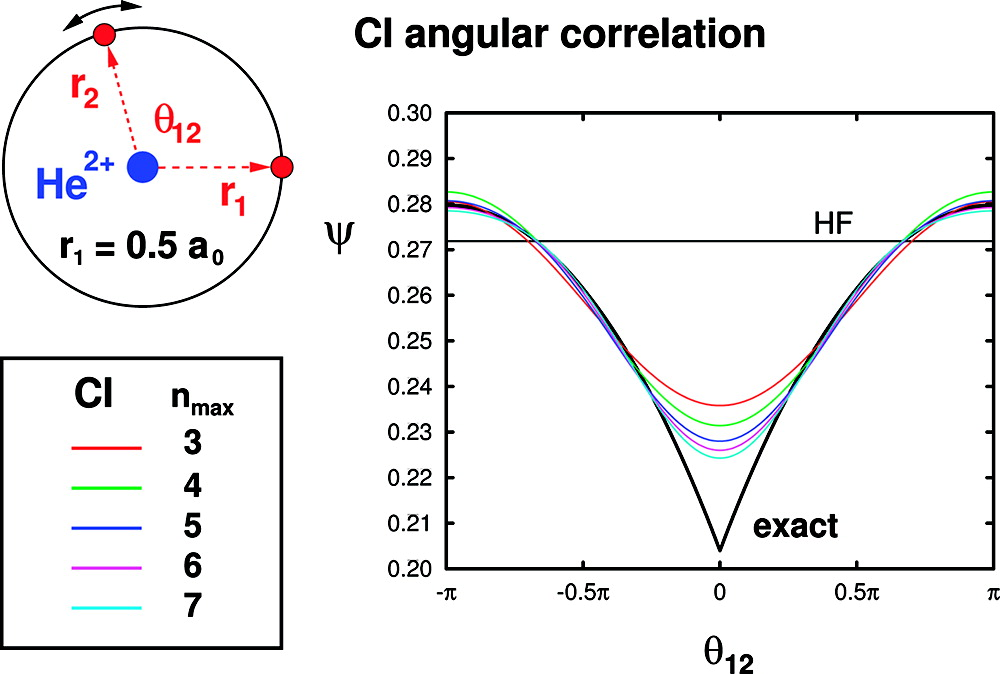
\includegraphics[width = 9cm, height = 6cm]{./pics/ang.jpeg}
        \caption{Electron-electron cusp condition for a Heliums ground state wave function with both electrons on the same circle of $.5 a_0$ using a CI based wave function with increasing basis size with maximum principle quantum number, $n_{max}$\cite{Hatting 2012}.}
    \end{figure}
    In order to more accurately calculate Coulombic correlation energy it is necessary to generate a new wave function expression that is explicitly dependent on inter-electronic distances. Kato's cusp condition\cite{kato 1957} comes from realizing the characterization of a first-order derivative discontinuity at the Coulombic type singularity\cite{Hatting 2012}. This fact provides the coalescence condition 
      \begin{equation}
          \left. \frac{\partial \Psi}{\partial r_{12}} \right |_{r_{12}=0} = - \frac{1}{2} \Psi(r_{12}=0)
        \end{equation}
    One assumes the form of the exact wave function is as follows:
      \begin{equation}
        \Psi_{exact}(r_1, r_2 , \dots) = \Phi(r_{12})\Psi(R_{12})
      \end{equation}
    Where $R_{12} \equiv \frac{r_1 + r_2}{2}$ and $r_{12} \equiv r_1 - r_2$ and the form of $\Phi{r_{12}}$ is chosen such that it satisfies the coalescence condition and 
      \begin{equation}
        \Phi(r_{12}) = R(r_{12})\Theta(\Omega_{12})
      \end{equation}
    The exact representation of the two electron portion, $\Phi(r_{12})$, can be solved through seperation of variables.  The angular portion, $\Theta(\Omega_{12})$, can be represented with the spherical harmonics, $Y_{lm}$, and the radial portion, $R(r_{12})$ can be solved using approximate solutions to the two-electron radial Schr{\"o}dinger equation
      \begin{equation}
        \left( -\frac{1}{2r^2_{12}} \frac{\partial}{\partial r_{12}} r^2_{12} \frac{\partial}{\partial r_{12}} + \frac{l(l+1)}{2r^2_{12}} + \frac{1}{r_{12}} + \mathcal{O}(r^0_{12}) \right) R(r_{12}) = 0
      \end{equation}
    Solving this differential with appropriate ans{\"a}tz provides the approximate solution
      \begin{equation}
        \Psi(r_1, r_2, \dots) \approx r^l_{12} \sum_{m=-l}^l\left( 1 + \frac{r_{12}}{2(l+1)} + \mathcal{O}(r^2_{12})\right) Y_{lm}(\Omega_{12})\Phi(R_{12},\dots)
      \end{equation}
    In the first attempts to create a wave function that was explicitly dependent on inter-electronic distances by Hartree \cite{Hartree 1928} and Hylleras\cite{Hylleras 1929}, the cusp condition was unknown and therefore the attempts could not effectively create functions that could be efficiently calculated.  Incorporation of cusp condition has allowed the introduction of functions many types of functions such as Hylleraas-CI, explicitly correlated Gaussian, and many body Gaussian geminal type.\cite{Kong 2012}  The development of these methods has allowed F12/R12 to develop as a computational tool.
    In the next sections I will discuss the use of F12/R12 in MP2 and CC methods.
    %Hartree and Ingman, the form used in modern F12/R12 methods.\\ %\cite{Hartree, D. R.; Ingman, A. L. Mem. Proc. Manchester Lit. Philos. Soc. 1933, 77, 69}
    \subsubsection{Explicitly Correlated MP2 R12 method}
      The formal difference between MP2 and MP2 R12 methods are the definition of first order wave function.  In standard MP2 theory the first order wave function is expressed as equation (32).  MP2-R12's first order wave function includes this term and explicitly correlated geminal functions.
        \begin{equation}
          \ket{\Psi_{MP2-R12}} = \ket{\Phi^(1)_{MP}} + \sum_{\substack{i<j \\ x<y}} t^{ij}_{xy} \ket{\Psi^{ij}_{xy}}
        \end{equation}
      Where the geminal basis function are quasi-double excitations with respect to the reference, $\ket{\Psi_0}$
        \begin{equation}
        \ket{\Psi^{ij}_{xy}} = \frac{1}{2} \bar{R}^{\alpha \beta}_{xy} \tilde{a}^{ij}_{\alpha \beta} \ket{\Psi_0}
        \end{equation}
      Where $\tilde{a}$ acting on the reference provides a doulby excited state and $\bar{R}^{\alpha\beta}_{xy}$ are matrix elements of the explicitly correlated factor, $f(r_{12})$ projected by a function, $\hat{Q}_{12}$, which ensure orthogonality of the excited geminal functions:
        \begin{equation}
          R^{\alpha \beta}_{xy} = \bra{\alpha \beta} \hat{Q}_{12} f(r_{12})\ket{xy}
        \end{equation}
      The most common choice for $\hat{Q}_{12}$, proposed by Valeev\cite{Valeev 2004} 
        \begin{equation}
          \hat{Q}_{12} = (1-\hat{O}_1)(1-\hat{O}_2)- \hat{V}_1 \hat{V}_2
        \end{equation}
      Other choices have also been considered \cite{wind 2002, Koppler 2002}.\\
      The doubly excited coefficients for the first order wave function can be solved for by minimizing Hylleraas functional for the second order MP energy 
        \begin{equation}
          H^{(2)} (\Phi^{(1)}) = \bra{\Phi^{(1)}} \hat{H}_0 - E_0 \ket{\Phi^{(1)}} + 2 \bra{\Phi}\hat{H}\ket{\Phi^{(0)}}
        \end{equation}
      using a modified one-step inversion of the zeroth Hamiltonian.  After solving for these coefficients $E_{\text{MP2-R21}}$ is 
        \begin{equation}
          E_{\text{MP2-R12}} = \bra{\Phi^{(0)}} \hat{H}^{(1)} \ket{\Phi^{1}} = E^{(2)}_{MP2} + E^{(2)}_{R12}
        \end{equation}
      The integrals of $E^{(2)}_{R12}$ can be solved analytically if the correlation factor, $f(r_{12})$, is Gaussian\cite{Polly 2006}.  The terms in $E^{(2)}_{R12}$ do require approximations to calculated fast and accurately some of which will be discussed later\cite{Kong 2012}.

    \subsubsection{Explicitly Correlated CC R12 method}
      It is necessary to apply R12 methods to CC in order to achieve the theories full potential because MP2-R12 has limited chemical framework\cite{kong 2012}.  CC-R12 extends the standard CC cluster operator, $\hat{T}$, to include R12 geminal operator, $f(r_{12})$\cite{Noga 1992, Noga 1994}